%%%%%%%%%%%%%%%%%%%%%%%%%%%%%%%%%%%%%%%%%%%%%%%%%%%%%%%%%%%%%%%%%%%%%%%%
% Plantilla TFG/TFM
% Escuela Politécnica Superior de la Universidad de Alicante
% Realizado por: Jose Manuel Requena Plens
% Contacto: info@jmrplens.com / Telegram:@jmrplens
%%%%%%%%%%%%%%%%%%%%%%%%%%%%%%%%%%%%%%%%%%%%%%%%%%%%%%%%%%%%%%%%%%%%%%%%

\chapter{Introduction}

This master’s thesis explores the application of computer vision and deep learning to the study of bird behavior and movement. By leveraging Python-based tools such as OpenCV, PyTorch, and scikit-learn, the project aims to develop an automated system for detecting, tracking, and analyzing bird motion from video data. The research also includes the creation of a web-based visualization platform, enabling interactive, geospatial exploration of behavioral patterns and habitat use, thus contributing to modern approaches in wildlife monitoring and conservation.
\\
\par The structure of that thesis chapter is organized as follows. Section 1.1 provides an overview of the research scope and background, while Section 1.2 outlines the motivation behind the study and its relevance to ecological monitoring. Section 1.3 presents the main goals and proposed technical approach. Section 1.4 describes the project timeline, including its key development stages, and Section 1.5 offers a brief outline of the overall thesis structure.

\section{Overview}

The increasing integration of artificial intelligence into scientific research has opened new possibilities for observing and understanding animal behavior. In particular, the use of video-based motion analysis has become a powerful tool in ornithology, enabling researchers to track bird movements with high precision and minimal intrusion. This thesis investigates the potential of modern deep learning and computer vision techniques to automate the detection, tracking, and analysis of bird activity using video data.

By combining tools such as OpenCV, YOLO, and PyTorch within a Python-based framework, the study aims to develop a scalable and efficient system for extracting behavioral insights from raw video footage. The project also includes the development of a web interface for visualizing movement data in a geospatial context. Overall, this work contributes to the interdisciplinary field of AI-assisted wildlife monitoring by offering practical methods and tools for data-driven ecological analysis. 

\section{Motivation}

Traditional methods of monitoring bird behavior — such as manual observation or tagging — are often limited in scale, accuracy, and continuity. They require significant human effort, can disturb natural behavior, and may fail to capture subtle patterns or long-term trends. With the rapid advancement of computer vision and deep learning, there is an opportunity to overcome these limitations by developing automated systems that can process large volumes of visual data efficiently and unobtrusively.

The motivation behind this thesis lies in bridging the gap between modern AI technologies and ecological field research. By enabling precise, continuous, and scalable tracking of birds in their natural environments, such systems can support biologists, conservationists, and researchers in gaining deeper insights into movement patterns, habitat preferences, and behavioral dynamics — ultimately contributing to more informed conservation efforts.

This research was also driven by an academic collaboration with the Languages and Computer Systems Department (Departamento de Lenguajes y Sistemas Informáticos, DLSI) and the Department of Computer Technology and Computing (Departamento de Tecnología Informática y Computación, DTIC). In particular, support from the 3D Perception Lab — an expert group in GPU acceleration, 3D computing, and computer vision — has provided valuable guidance and resources. The group is actively involved in the national MoDeAss project (Monitoring and Detection of Human Behaviors for Personalized Assistance and Early Disease Detection, known as A2HUMPA in Spanish), led by Professor José García Rodríguez. Their technical expertise and infrastructure played an essential role in shaping the direction and feasibility of this thesis.

On a more personal level, I have always had a strong interest in animals, particularly birds, and their complex behaviors. This thesis represents a unique opportunity to combine that long-standing fascination with my passion for technology and computer science to part of the nature. It offers a meaningful way to explore how modern computational tools can be applied to better understand and protect the natural world.

\section{Proposal and goals}

The main proposal of this thesis is to design and implement an automated system for capturing, tracking, and analyzing the movement of birds using video data and modern deep learning techniques. The system is intended to operate efficiently on real-world recordings, extracting motion patterns and behavioral features in a way that minimizes the need for manual intervention.

To achieve this, the project sets the following key goals:

\begin{itemize}
    \item \textbf{Detection and Tracking:} Implement a reliable pipeline for identifying and tracking birds in video footage using models such as YOLO for object detection and DeepSORT for multi-object tracking.
    \item \textbf{Data Processing and Analysis:} Extract and structure movement data to enable further behavioral analysis, including trajectory visualization and statistical evaluation.
    \item \textbf{Tool Integration:} Leverage Python-based tools and libraries---such as OpenCV, PyTorch, scikit-learn, and pandas---for efficient data handling, model deployment, and preprocessing.
    \item \textbf{Visualization Platform:} Develop an interactive web-based interface using Flask and CesiumJS to display geospatial movement data and behavioral statistics in an accessible format.
    \item \textbf{Scientific Contribution:} Provide a modular and extensible system that can be adapted for broader applications in ecological monitoring and contribute to interdisciplinary research combining AI and wildlife studies.
\end{itemize}

These goals guide the structure and implementation of the thesis, ensuring both technical depth and ecological relevance.


\section{Timeline}

The timeline of this thesis spans from September 2024 to August 2025 and is divided into four main stages: Learning, Research, Implementation, and Experimentation. These stages reflect a logical and gradual development process, starting from acquiring theoretical knowledge, moving through technical investigation, system development, and finally, rigorous evaluation. This structure ensures that each phase builds upon the outcomes of the previous one, allowing for a coherent and well-structured progression of the work. The full schedule of tasks and milestones is illustrated in the Gantt chart presented in Figure 1.1.

\begin{figure}[H]
	\centering
	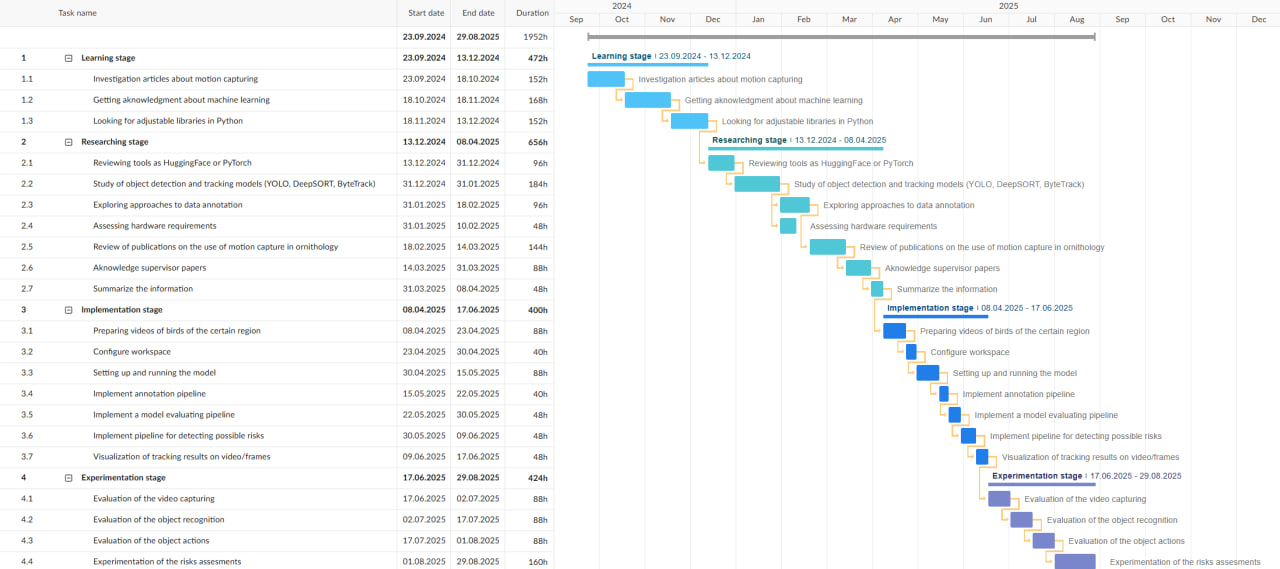
\includegraphics[width=0.8\textwidth]{archivos/figuras/gantt-chart.jpg}
	\caption{Gantt chart illustrating the timeline of the thesis project.}
	\label{fig:gantt-chart}
\end{figure}

\subsection{Learning stage}

The Learning stage takes place from September to December 2024. During this period, the focus is on acquiring the theoretical foundation required for the project. This includes investigating academic literature on motion capturing, developing a general understanding of machine learning principles, and exploring available Python libraries that could be used for computer vision and deep learning tasks. Special attention is given to the capabilities of OpenCV and YOLO, as they are expected to form the technical backbone of the detection and tracking pipeline.

\begin{figure}[H]
	\centering
	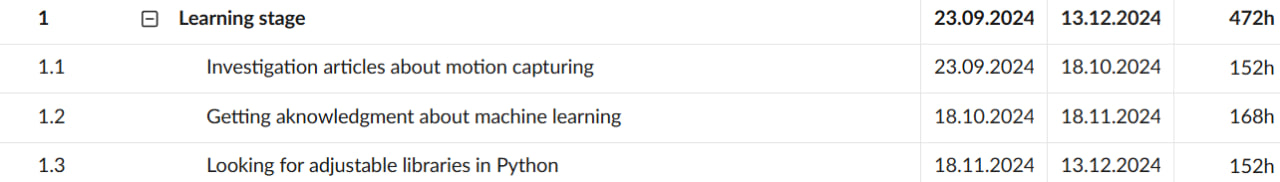
\includegraphics[width=0.8\textwidth]{archivos/figuras/learning-stage.jpg}
	\caption{Learning stage: foundational knowledge acquisition.}
	\label{fig:learning-stage}
\end{figure}
	
\subsection{Research stage}

The Research stage runs from December 2024 to April 2025. This phase deepens the technical understanding established earlier by examining specific tools such as Hugging Face, PyTorch, and annotation platforms. It also involves studying advanced object detection and tracking models (YOLO, DeepSORT, ByteTrack), comparing their strengths and limitations. Additional tasks include assessing the computational requirements for running deep learning workloads, reviewing scientific literature on the use of motion capture in ornithology, and becoming familiar with the supervisor’s related publications. This stage concludes with a synthesis of all the gathered knowledge, which informs the design of the system.

\begin{figure}[H]
	\centering
	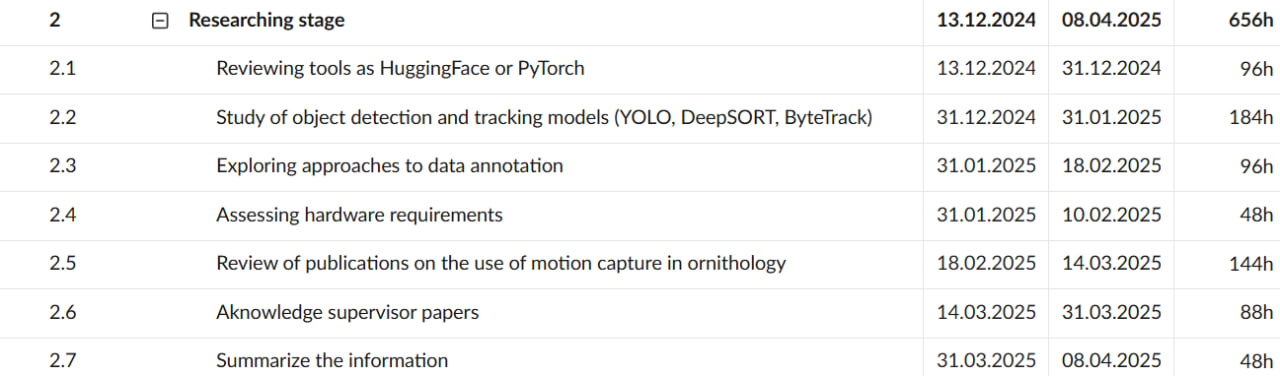
\includegraphics[width=0.8\textwidth]{archivos/figuras/research-stage.jpg}
	\caption{Research stage: in-depth exploration of models and techniques.}
	\label{fig:research-stage}
\end{figure}

\subsection{Implementation stage}

The Implementation stage is scheduled for April to June 2025. This is the core development phase of the project, where theoretical insights are transformed into a working system. It involves preparing video data of birds, setting up the programming and hardware environment, configuring and running selected models, and developing annotation, evaluation, and risk detection pipelines. The goal is to build a functional and modular processing system that automates key parts of the data analysis workflow. In addition, the first version of a visual interface for displaying tracking results will be produced.

\begin{figure}[H]
	\centering
	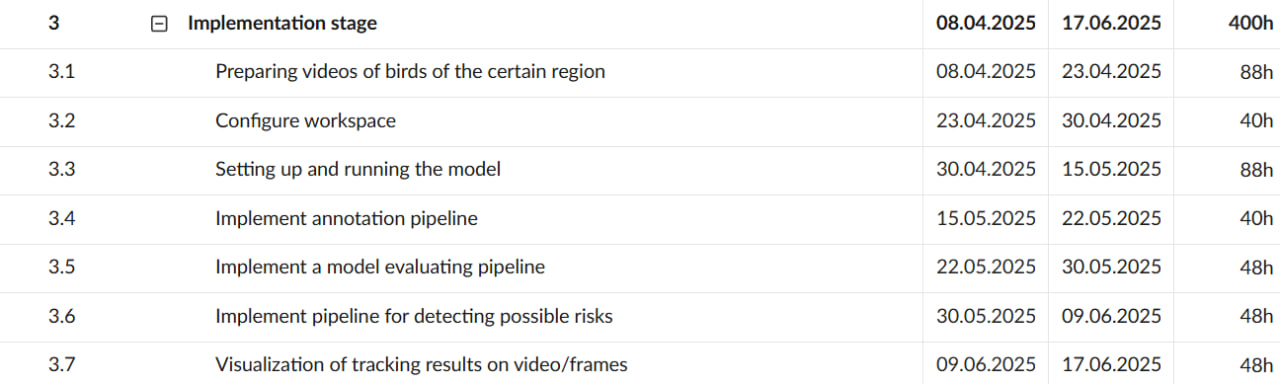
\includegraphics[width=0.8\textwidth]{archivos/figuras/implementation-stage.jpg}
	\caption{Implementation stage: practical realization of the system.}
	\label{fig:implementation-stage}
\end{figure}

\subsection{Experimentation stage}

The final Experimentation stage takes place from June to August 2025. In this phase, the developed system is tested on real-world or simulated video datasets. Experiments are conducted to evaluate the quality of video input, accuracy of object detection and tracking, behavioral recognition capabilities, and the performance of the risk detection module. The results are documented and analyzed both quantitatively and visually. This stage helps validate the effectiveness of the system and provides the basis for drawing final conclusions.

\begin{figure}[H]
	\centering
	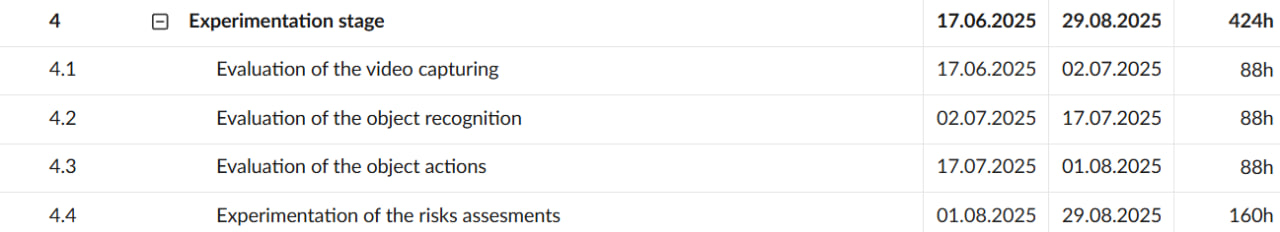
\includegraphics[width=0.8\textwidth]{archivos/figuras/experimentation-stage.jpg}
	\caption{Experimentation stage: performance assessment of the system.}
	\label{fig:experimentation-stage}
\end{figure}

\section{Outline}

This thesis is structured into six main chapters. The remainder of the document is organized as follows: Chapter 2 provides a comprehensive review of the current techniques, models, and datasets relevant to Video Captioning, forming the foundation for the subsequent work. Chapter 3 details the infrastructure and technologies employed during experimentation. In Chapter 4, we describe the various reference components utilized in the study. Chapter 5 presents the proposed architectures along with their evaluation results. Finally, Chapter 6 offers a summary of the key contributions and discusses potential directions for future research, bringing the thesis to a close.


 
 



